% !TEX root = ../gen_report.tex
\section{Цель работы}
Получить практические навыки работы с БД путем создания собственного интерактивного генератора
данных на языке программирования python.

\section{Ход работы}
Была создана команда \textbf{generate}, которая имеет два входных параметра:

\begin{enumerate}
	\item \textbf{table} --- название таблицы или области для которой необходимо сгенерировать данные. В случае ввода \textbf{all} произойдет генерация для всех таблиц.
	\item \textbf{count} --- целочисленное число, обозначающее количество строк, которое необходимо сгенерировать.
\end{enumerate}

Данные генерируются случайным образом в виде случайных чисел, времени, дат и строк, состоящих из случайных символов (заглавные английские буквы и цифры).

Также присутствует возможность генерации данных для таблиц из одной области (\vref{fig:db_scheme}).

\begin{figure}[H]
	\centering
	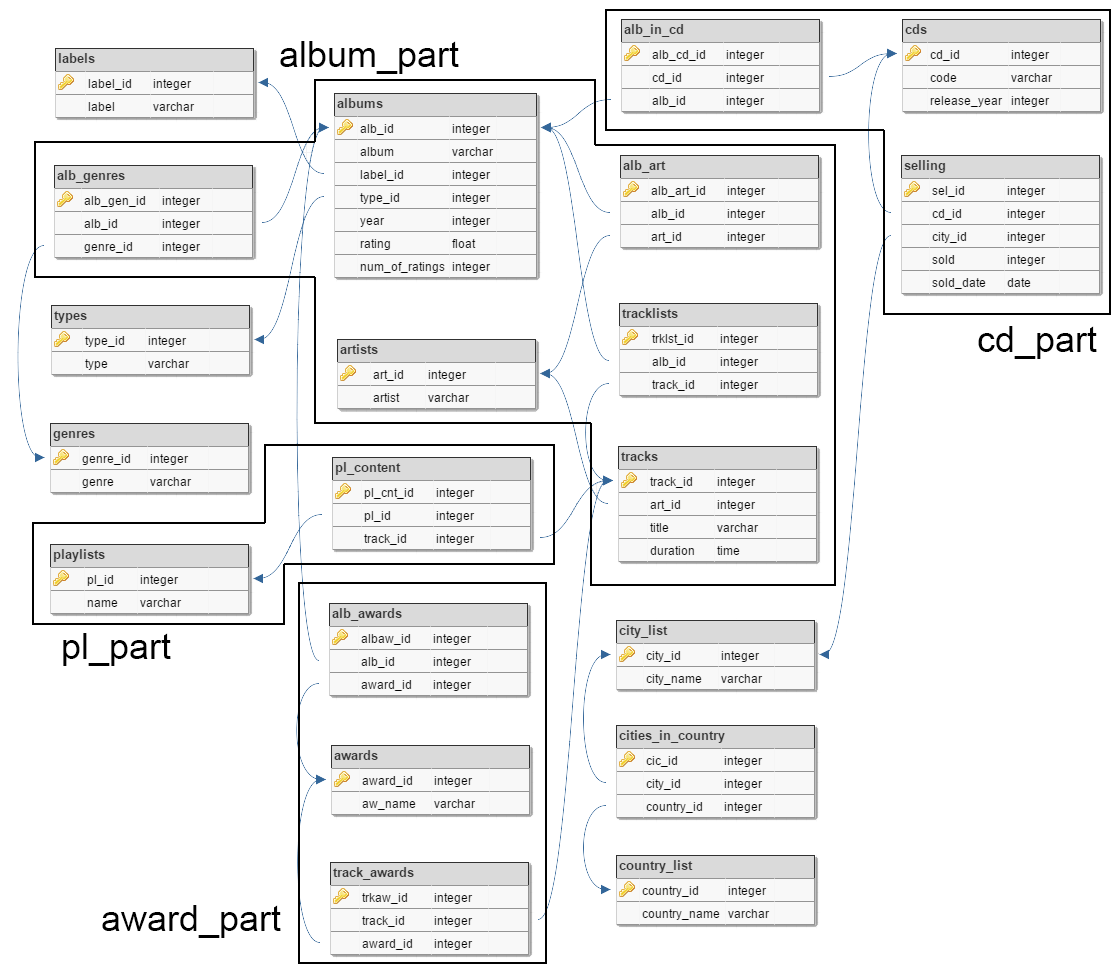
\includegraphics[width=0.9\textwidth]{scheme_m2}
	\caption{SQL-схема БД}
	\label{fig:db_scheme}
\end{figure}

Для каждой из областей также задается параметр count, однако для таблиц, состоящих в области, данный коэффициент модифицируется следующим образом:

\begin{enumerate}
	\item cd\_part
	\begin{itemize}
		\item cds $\rightarrow$ count
		\item alb\_in\_cd $\rightarrow$ count $\times$ 3
		\item selling $\rightarrow$ count $\times$ 2
	\end{itemize}
	\item album\_part
	\begin{itemize}
		\item albums $\rightarrow$ count
		\item alb\_genres $\rightarrow$ count $\times$ (1 || 2) 
		\item artist $\rightarrow$ count
		\item tracks $\rightarrow$ count $\times$ 5
		\item alb\_art $\rightarrow$ count $\times$ (1 || 2)
		\item tracklists $\rightarrow$ count $\times$ 5
	\end{itemize}
	\item award\_part
	\begin{itemize}
		\item awards $\rightarrow$ count
		\item alb\_awards $\rightarrow$ count $\times$ 2
		\item track\_awards $\rightarrow$ count  $\times$ 4
	\end{itemize}
	\item pl\_part
	\begin{itemize}
		\item playlists $\rightarrow$ count
		\item pl\_content $\rightarrow$ count $\times$ 5
	\end{itemize}
\end{enumerate}

Пример использования команды для генерации 5 новых строк в каждую из таблиц базы данных приведен в листинге \vref{adding}.

\begin{lstlisting}[label=adding,caption=Пример иcпользования команды]
D:\4 course\lastsem\db\lab1\lab1>python manage.py generate all 5
5 row(s) addded to cds.
5 row(s) addded to labels.
5 row(s) addded to types.
5 row(s) addded to genres.
5 row(s) addded to artists.
5 row(s) addded to tracks.
5 row(s) addded to playlists.
5 row(s) addded to pl_content.
5 row(s) addded to albums.
5 row(s) addded to alb_genres.
5 row(s) addded to alb_in_cd.
5 row(s) addded to alb_art.
5 row(s) addded to tracklists.
5 row(s) addded to awards.
5 row(s) addded to track_awards.
5 row(s) addded to alb_awards.
5 row(s) addded to city_list.
5 row(s) addded to country_list.
5 row(s) addded to cities_in_country.
5 row(s) addded to selling.
\end{lstlisting}

\section{Вывод}
В ходе данной работы было продолжено создание приложения, работающего с базой
данных, путем разработки генератора данных. Собственная реализация в отличие от встроенных в какие-либо СУБД генераторов получается более удобной и гибкой, позволяя дополнять и изменять ее при необходимости.

Генератор случайных строк получается достаточно быстрым по производительности. На время генерации влияют проверки на возможность генерации данных (например, определение диапазона доступных записей по внешнему ключу и проверка на наличие записей в таблице, так как для получения этих данных используются запросы к БД).